In this section we present a method for extracting behavioural~\emph{scenarios}
from system control programs and synthesising hardware microcontrollers that can
execute these scenarios. We rely on Conditional Partial Order Graphs
(CPOGs)~\cite{CPOG} and associated tool support for synthesis; specifically, we
use the CPOG plugin~\cite{scenco-tool} of the~\textsc{Workcraft}
framework~\cite{workcraft-tool}, which provides support for scenario
specification and synthesis, and handles the translation of CPOGs to circuits
to produce a physical implementation of the system microcontroller.

\subsection{Extracting scenarios from programs}

We define a \textit{scenario} as a \textit{partial order}~(PO)
$(\mathcal{I},\prec)$, i.e. a binary precedence relation~$\prec$ defined on a
set of instructions $\mathcal{I}$ that satisfies two properties~\cite{PO}:

\begin{itemize}
    \item Irreflexivity: $\forall a \in \mathcal{I}, \neg(a \prec a)$
    \vspace{+1mm}
    \item Transitivity: $\forall a, b, c \in \mathcal{I}, (a \prec b) \wedge (b
    \prec c) \Rightarrow (a \prec c)$
\end{itemize}

To extract scenarios from programs, we reuse the dependency analysis that we
developed for implementing concurrency oracles in the previous section. As one
can see from our definition of scenarios, we only require to keep the
information about the (partial) ordering of instructions. We can therefore
discard the unnecessary details about which particular register, flag or memory
location was the cause of the dependency, leading to the following procedure.

\vspace{-5mm}
\subsubsection{Extracting the behavioural scenario from a program:}
\begin{enumerate}
\vspace{-2mm}
    \item Calculate all static data dependencies between the program instructions.
    \item Construct the static dependency graph.
    \item Contract data vertices, keeping the induced arcs between the instructions.
    \item Perform the \emph{transitive closure} of the resulting graph.
\end{enumerate}

\subsection{Scenario encoding and synthesis}

In the context of this paper, we consider control systems which are programmed
in low-level assembly-like languages. Using the procedure from the previous subsection,
we can extract behavioural scenarios, represented as partial orders, from the
system's control programs. These partial orders often have some shared
functionality, which can be exploited by Conditional Partial Order Graphs and
associated synthesis methods, leading to more efficient hardware implementations
compared to those obtained by implementing each scenario separately.

\vspace{-5mm}
\subsubsection{Microcontroller synthesis:}
\begin{enumerate}
\vspace{-2mm}
    \item Extract the scenarios from a given set of system control programs.
    \item Synthesise a CPOG containing all the scenarios.
    \item Apply the CPOG workflow for optimisation and compilation to hardware.
\end{enumerate}

% The Conditional Partial Order Graphs formalism is supported in the open source
% framework Workcraft, which facilitates construction and visualisation of partial
% orders, their synthesis into a CPOG and compilation to logical circuits.

In the next subsection we will illustrate the described microcontroller
synthesis approach on a simple example. We will consider a system with two
control programs, extract the scenarios from these programs and synthesise them
into a CPOG with some shared functionality.

\vspace{-3mm}
\subsection{Example}

To illustrate the use of the scenario extraction procedure, let us sketch an
example of a system controlling a hypothetical dual-motor autonomous vehicle.
The vehicle has two motors directly driving its left and right front wheels.
The system control unit has a simple application-specific instruction set, two
general-purpose registers and a memory unit with four cells. The input to the
unit is provided in memory cells 0 and 1. The unit controls the velocity of the
left and right motors by outputting values to the cells 2 and 3, respectively.
A motor's velocity may be adjusted with the instruction~\hs{Adjust} supplying
the input value in a register and referring a target motor (2 or 3).

The first program (Fig.~\ref{fig-scenarios-drive-straight}, left) implements
the ``drive straight'' behaviour, driving both wheels with the same velocity.
The graph on the right pictures the extracted partial order.

\begin{figure}[H]
\centering
\begin{minipage}[b]{0.5\textwidth}
\begin{minted}[linenos,xleftmargin=50pt]{haskell}
Load R0 0
Adjust R0 2
Adjust R0 3
\end{minted}
\vspace{5mm}
\end{minipage}
% \hfill
\begin{minipage}[b]{0.4\textwidth}
\includegraphics[scale=0.35]{img/ataed-scenario-drive-straight.pdf}
\end{minipage}
\vspace{-3mm}
\caption{Scenario ``drive straight'' and the corresponding
partial order.\label{fig-scenarios-drive-straight}}
\vspace{-7mm}
\end{figure}

Another behaviour is ``drive and turn'', which is implemented by adjusting the
velocities with different values (Fig.~\ref{fig-scenarios-turn}). In this case,
the resulting partial order contains two independent components.

\begin{figure}[H]
\vspace{-5mm}
\centering
  \begin{minipage}[b]{0.5\textwidth}
\begin{minted}[linenos,xleftmargin=50pt]{haskell}
Load R0 0
Load R1 1
Adjust R0 2
Adjust R1 3
\end{minted}
\vspace{3mm}
\end{minipage}
% \hfill
\begin{minipage}[b]{0.4\textwidth}
\includegraphics[scale=0.35]{img/ataed-scenario-turn.pdf}
\end{minipage}
\vspace{-3mm}
\caption{Scenario ``drive and turn'' and the corresponding
partial order.\label{fig-scenarios-turn}}
\vspace{-8mm}
\end{figure}

\begin{figure}[H]
\vspace{-5mm}
\centerline{\includegraphics[scale=0.35]{img/ataed-composition.pdf}}
\vspace{-2mm}
\caption{Two operation scenarios and their composition.\label{fig-scenarios-composition}}
\vspace{-7mm}
\end{figure}

Fig.~\ref{fig-scenarios-composition} displays the Conditional Partial
Order Graph which represents the composition of the two scenarios, where the
additional control input \textsf{x\_0} is used to select the active scenario.
The partial orders extracted from the programs are efficiently merged, thus
rendering the CPOG composition to be more compact then a simple list of the
extracted scenarios. The resulting hardware microcontroller, mapped to a 2-input
gate library, is shown in Fig.~\ref{fig-scenarios-circuit}.

\begin{figure}[h]
\vspace{-5mm}
\centerline{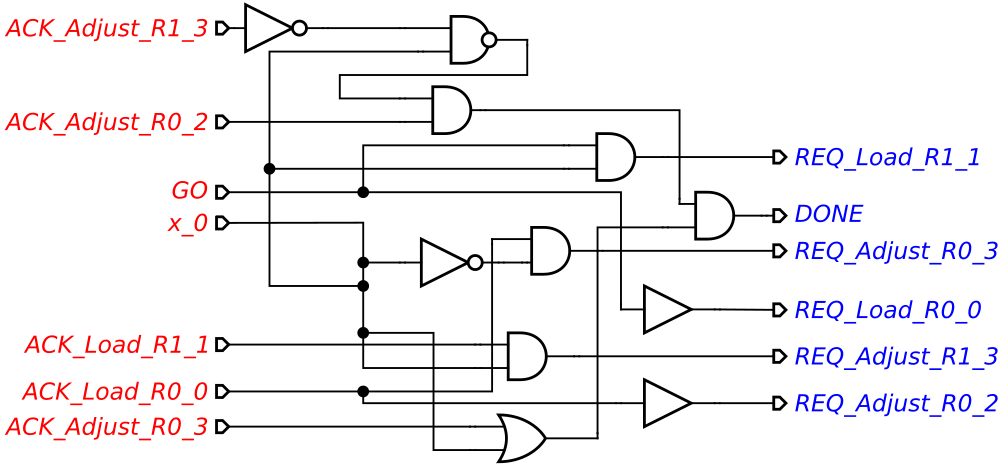
\includegraphics[scale=0.4]{img/ataed-circuit.pdf}}
\vspace{-3mm}
\caption{Synthesised hardware microcontroller.\label{fig-scenarios-circuit}}
\vspace{-7mm}
\end{figure}

